\clearpage
\makeatletter
\efloat@restorefloats
\makeatother


\begin{appendix}
\section{}
Additional analyses were conducted in an attempt to clarify the effect
of task on classification accuracy. These supplementary analyses were
not seen as central to the current study, but could prove to be
informative to researchers attempting to replicate or extend these
findings in the future. The results from the primary analysis showed
that classification accuracies were the lowest for the Memorize
condition. To further understand why classification accuracy was lower
for the Memorize condition than it was for the Search or Rate condition,
the Exploratory and Confirmatory timeline datasets were systematically
batched into subsets with the Search (S), Memorize (M), or Rate (R)
condition removed (i.e., \(\varnothing\)MR, S\(\varnothing\)R,
SM\(\varnothing\)).

All of the data subsets analyzed in this supplementary analysis were
decoded with better than chance accuracy (see Figure
@ref(fig:supp-chance)a). The same pattern of results was observed in
both the Exploratory and Confirmatory datasets. When the Memorize
condition was removed, classification accuracy improved (see Table
@ref(tab:supp-comparisons); see Figure @ref(fig:supp-chance)a). When the
Rate condition was removed, classification was the worst. When the
Memorize condition was included (i.e., SM\(\varnothing\) and
\(\varnothing\)MR), mis-classifications were biased toward Memorize, and
the Memorize condition was more accurately predicted than the Search and
Rate conditions (see Figure @ref(fig:supp-conf-matrices)).

\begin{figure}
\centering
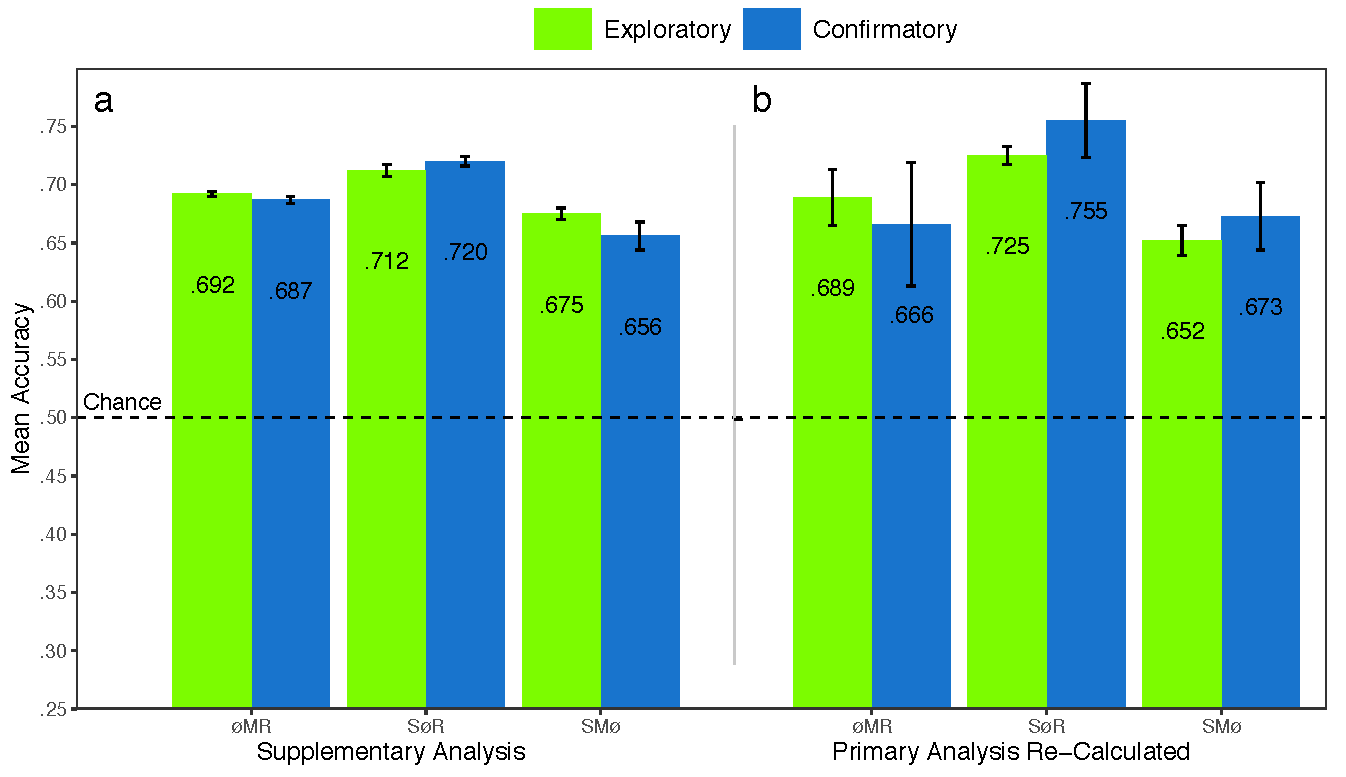
\includegraphics{figures/supp_analysis/supp_subset_chance.pdf}
\caption{(\#fig:supp-chance)The graph represents the average accuracy
reported for each subset of the Exploratory and Confirmatory timeline
data for (a) the re-calculated accuracies from the primary analysis, and
(b) the supplementary analysis. All of the data subsets were decoded at
levels better than chance (.50). The error bars represent standard
errors.}
\end{figure}

\begin{table}[!h]
    \centering
    \caption{Supplementary Subset Comparisons}
    \label{tab:supp-comparisons}
    \begin{tabular}{l c c c c}
         & \multicolumn{2}{c}{Exploratory} & \multicolumn{2}{c}{Confirmatory} \\
        \hline
        Comparison & \textit{t} & \multicolumn{1}{c|}{\textit{p}} & \textit{t} & \textit{p} \\
        \hline
        $\varnothing$MR vs. S$\varnothing$R & 3.248 & \multicolumn{1}{c|}{.008} & 3.094 & .012 \\
        $\varnothing$MR vs. SM$\varnothing$ & 2.875 & \multicolumn{1}{c|}{.021} & 2.923 & .018 \\
        S$\varnothing$R vs. SM$\varnothing$ & 6.123 & \multicolumn{1}{c|}{< .001} & 6.017 & < .001 \\
        \hline
    \end{tabular}
\end{table}

\begin{figure}
\centering
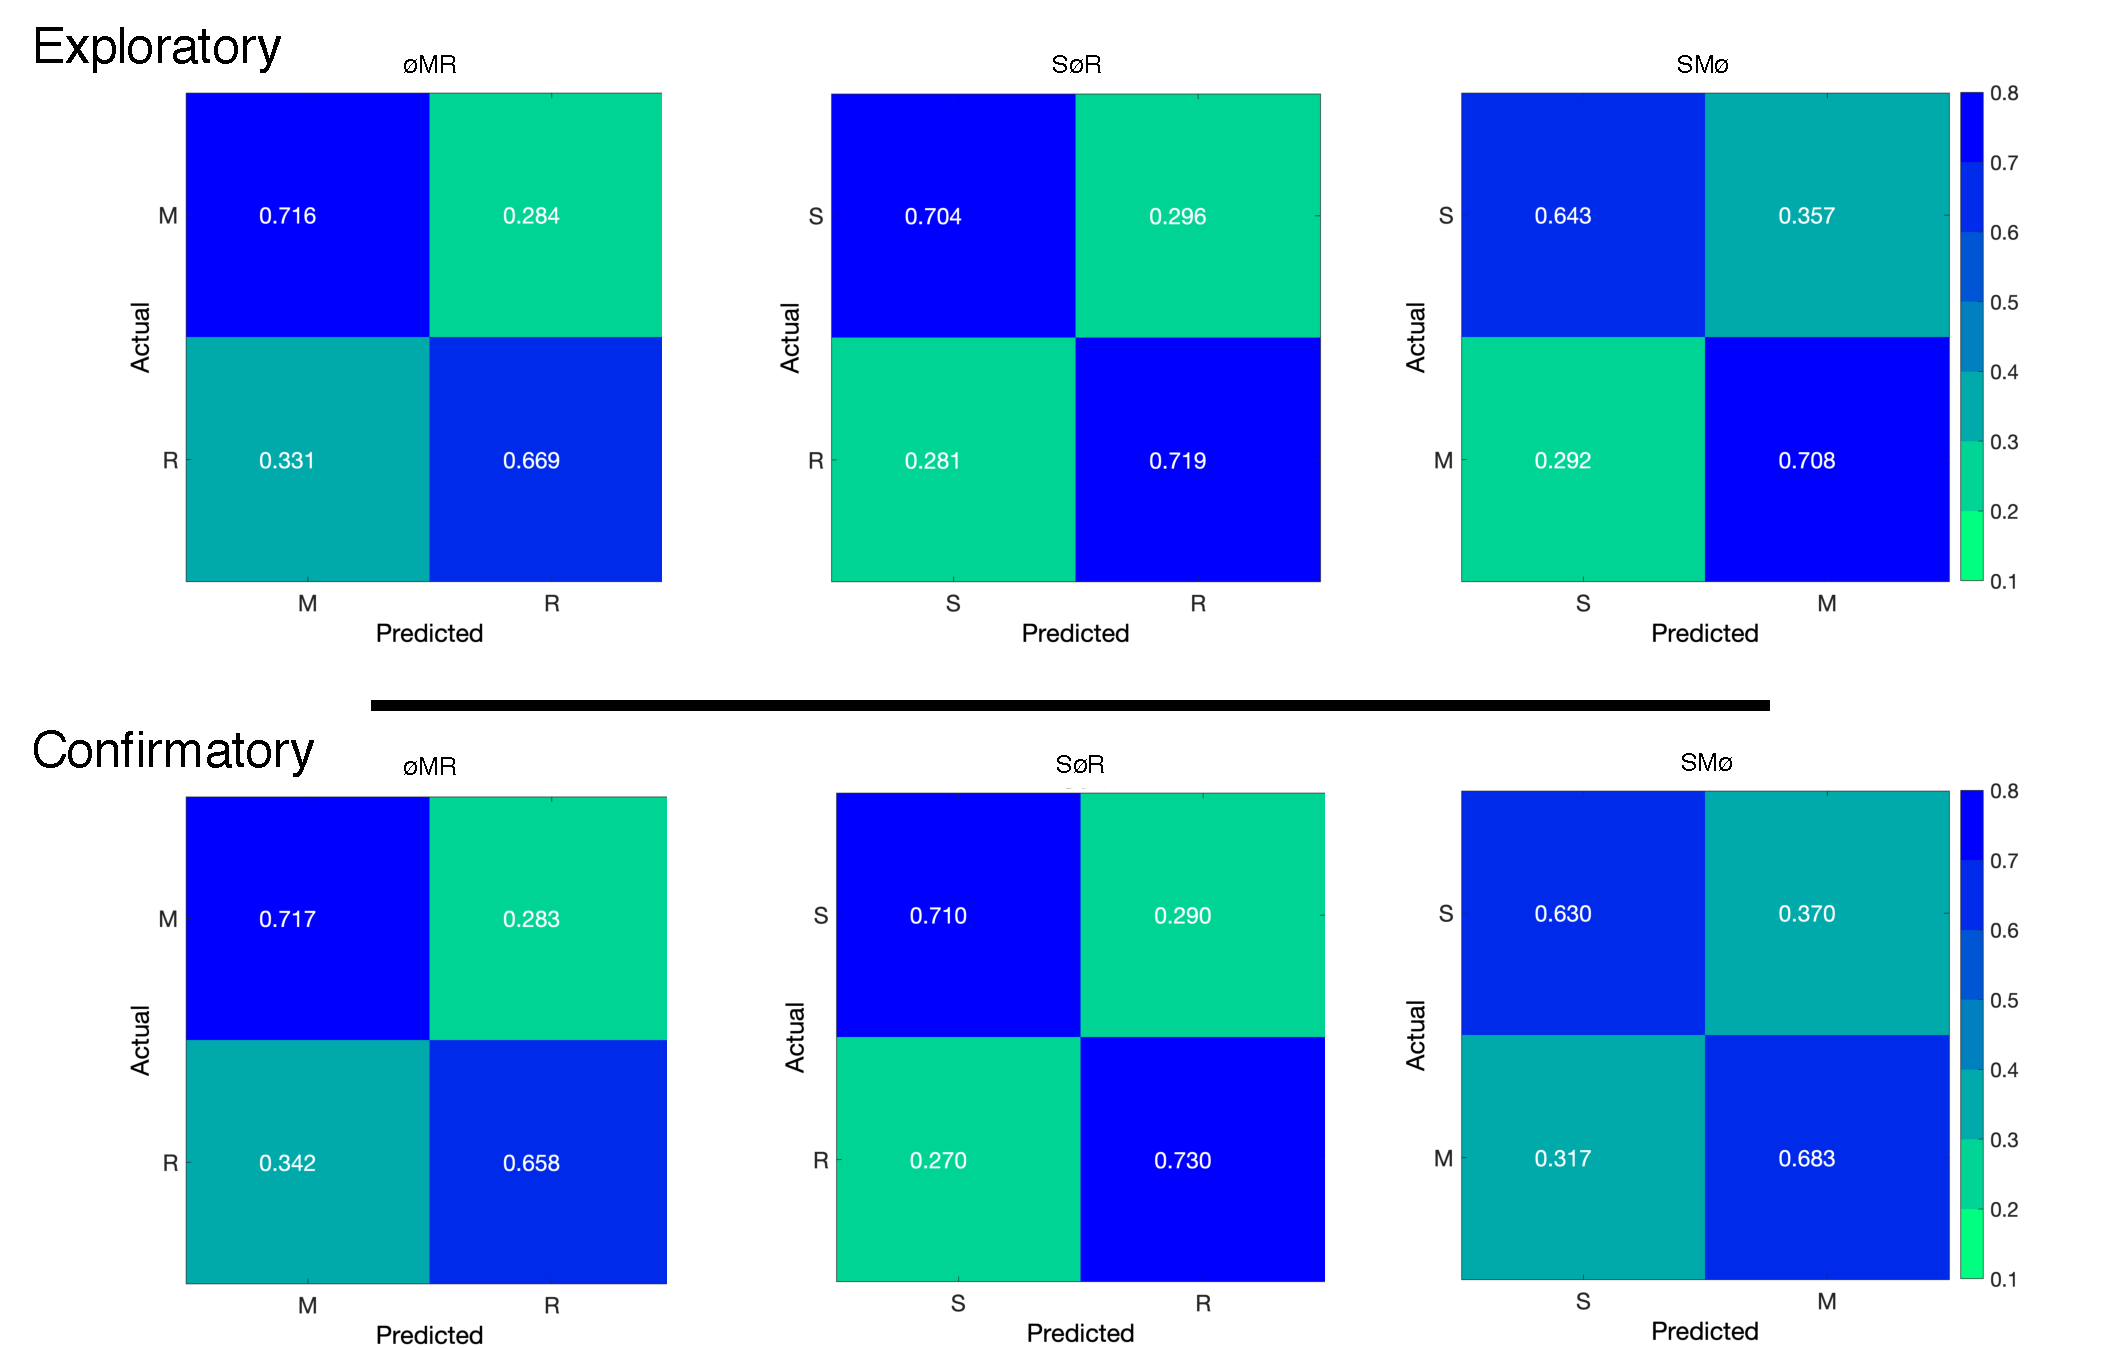
\includegraphics{figures/supp_analysis/confusion_matrices/supp_conf_matrices.pdf}
\caption{(\#fig:supp-conf-matrices)The confusion matrices represent the
average classification accuracies for each condition of the timeline
data (S = Search, M = Memorize, R = Rate). The vertical axis of the
confusion matrices represents the actual condition for the trial. The
horizontal axis of the confusion matrices represents the condition that
was predicted by the model.}
\end{figure}

The accuracies for all of the data subsets observed in the supplementary
analysis were higher than the accuracies observed in the main analysis.
Although there is a clear difference in accuracy, the primary analysis
was classifying three categories (chance = .33) and the supplementary
analysis was classifying two categories (chance = .50). Because the
baseline chance performance was different for the primary and
supplemental analyses, any conclusions drawn from a comparison of the
results of analyses could be misleading. For this reason, we revisited
the results from the primary analysis and re-calculated the predictions
to be equivalent to a 50\% chance threshold. Because the
cross-validation scheme implemented by the DeLINEATE toolbox
(\href{https://delineate.it}{htpps://delineate.it}; Kuntzelman et al.,
under review) guaranteed an equal number of trials in the test set are
assigned to each condition for each dataset, we were able to
re-calculate 2-category predictions from the 3-category predictions
presented in the confusion matrices from the primary analysis (see
Figure @ref(fig:timeline-conf-matrices)). The predictions were
re-calculated using the following formula:
Prediction\(_{(A, A, A\varnothing C)}\) = Prediction\(_{(A, A, ABC)}\) /
(Prediction\(_{(A, A, ABC)}\) + Prediction\(_{(A, C, ABC)}\)). For
example, accuracy for the Search classification for S\(\varnothing\)R
would be calculated with the following:
Prediction\(_{(S, S, S\varnothing R)}\) =
Prediction\(_{(S, S, S\varnothing R)}\) /
(Prediction\(_{(S, S, S\varnothing)}\) +
Prediction\(_{(S, R, S\varnothing R)}\), where
Prediction\(_{(S, R, S\varnothing R)}\) is the ratio of Search trials
that were misclassified as Rate.

The results for the re-calculated predictions followed a pattern similar
to the supplementary analysis (see Figure @ref(fig:supp-chance)b). This
is supported by the persisting tendancy of the algorithm to mis-classify
Search and Rate trials in the SM\(\varnothing\) and \(\varnothing\)MR
subsets as Memorize (see Figure @ref(fig:recalc-conf-matrices)). Looking
back at the primary analysis, the 3-category classifications predicted
the Memorize conditions with the lowest accuracy (c.f., Search and Rate
conditions), mis-classifications of the Search and Rate conditions were
most often categorized as Memorize (see Figure
@ref(fig:timeline-conf-matrices)). This overall pattern points toward a
general bias to categorize uncertain trials as Memorize.

\begin{figure}
\centering
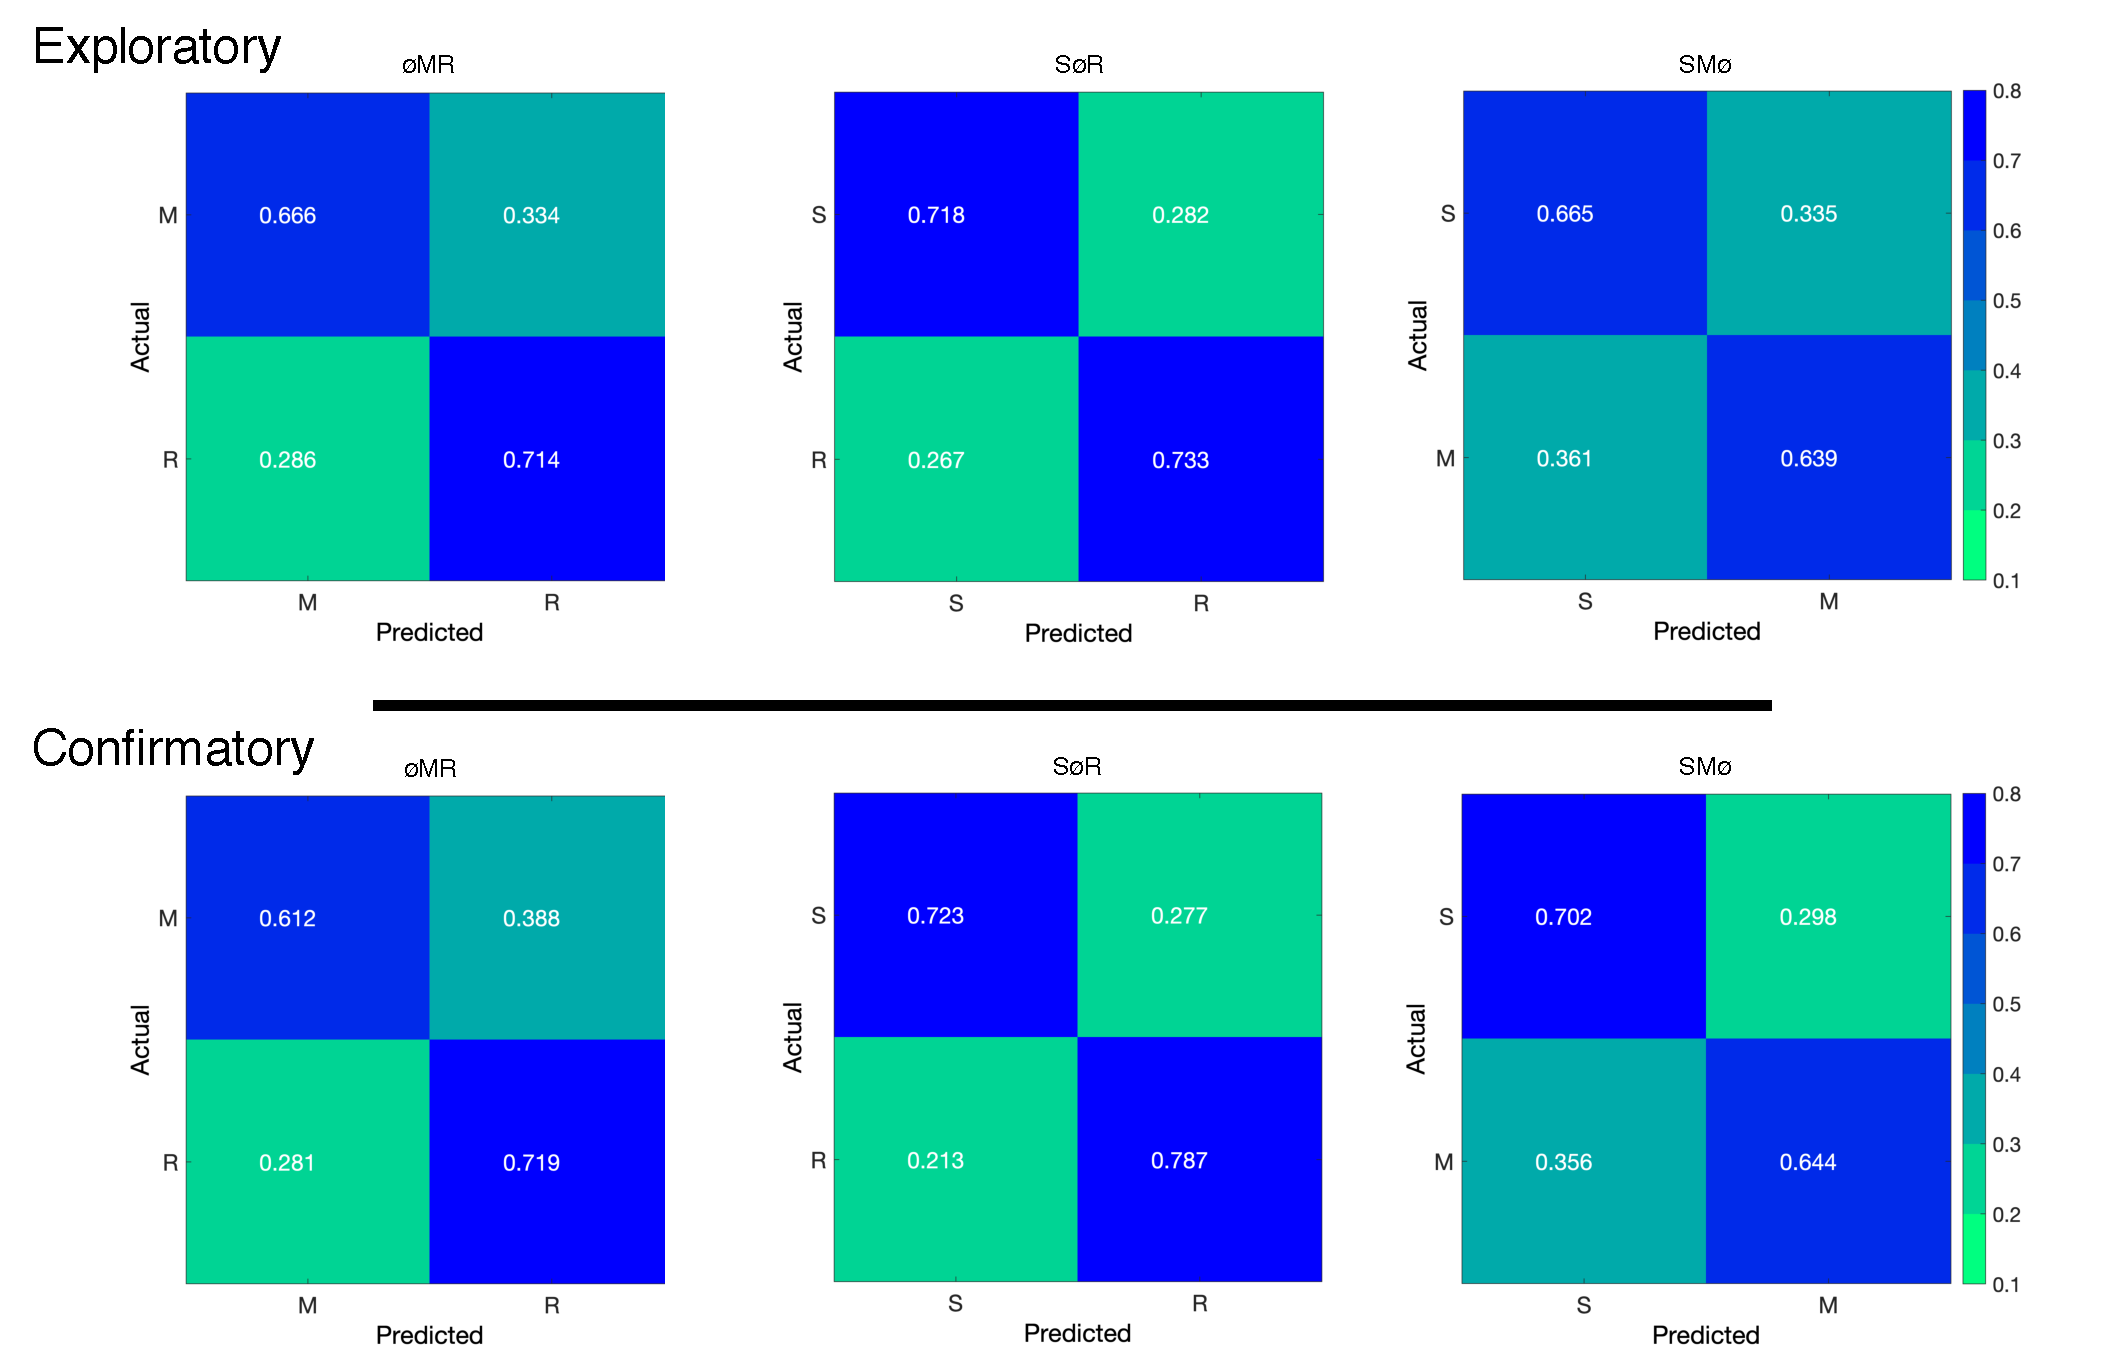
\includegraphics{figures/supp_analysis/recalculations/confusion_matrices/recalc_conf_matrices.pdf}
\caption{(\#fig:recalc-conf-matrices)The confusion matrices represent a
re-calculation of the classification accuracies for each category from
the primary analysis. This re-calculation is meant to make the
accuracies presented in the primary analysis (chance = .33) equivalent
to the classification accuracies presented in the supplementary analysis
(chance = .50).}
\end{figure}
\end{appendix}
